\section{Solvable representations}

\begin{displayquote}
  \textit{Abstraction for efficient optimisation.}
\end{displayquote}

{\color{red}This whole intro section!?!?}

% bellman eqn is hard to solve (how hard?)
Existing solvers of MDPs such as are not efficient: value iteration requires at
least \href{https://en.wikipedia.org/wiki/EXPTIME}{EXPTIME} iterations,
policy iteration requires ???, or policy gradients,
require a ??? amount of computation.
Yet, recent work \cite{} has shown that MDPs require at least $\Omega(|S|^2|A|).$

% (lower bound computational complexity?!)
Is there a way to turn this into an easier problem to solve?

% maybe we can find an abstraction that allows more powerful solvers?

% what are more powerful sovlers?
Well, which problems are easy to solve? Convex ones, linear ones, continuous ones, ... \cite{ODonoghue2012a}

% how can we use these more powerful solvers for RL?
So, is it possible to convert the
 linear problem? What sacrifices need to be made to
achieve this?

\subsection{Linear Markov decision problems (LMDPs)}

\begin{displayquote}
Why linear?
\end{displayquote}

% How are we exploiting linearity?
% Linearisation around the optima? Intuition. How to see this? Stephen!?
Intuition.

\subsubsection{Existing linear methods}

% many mathematical tools for analysis.
% we know linear systems can be solved efficiently.

% Linearity in MDPs
% Polytope. LPs


\subsubsection{Compositionality}

Imagine if your life were linear, in the sense of effort and achieving goals.
More work in equals proportionally more rewards. This makes decision making
a lot more simple. Pick the most rewarding ???, and work hard.

Saxe el al. observe the power of linearity: \textit{"Consider two standard MDPs
$M_1 = \{S, A, P, R_1\}$ and $M_2 = \{S, A, P, R_2\}$ which have
identical state spaces, action sets, and transition dynamics but differ in their
instantaneous rewards $R_1$ and $R_2$. These may be solved independently to
yield value functions $V_1$ and $V_2$. [If the problems were linear then] the value function of the MDP
$M_{1+2} = \{S, A, P, R_1 +R_2\}$, whose instantaneous rewards are the sum of the
first two, [would be] $V_{1+2} = V_1 + V_2$.} \cite{Saxea}

% why do we care about multitask!?
The ability to recycle knowledge from a task to a new task is !!!



% are there other famous examples of linearising something to make it easy to solve?!?

\subsubsection{What do we mean by a linear MDP?}

Do we mean that the value function is a linear function of the policies,
of the reward function, of the transition function? Others have tried to incorporate
linearity into MDPs in a few different ways.

\begin{itemize}
  \tightlist
  \item Jin et al. construct a MDP where the value is a linear function of a state-action representation. \cite{Wang}
  \item Levine et al. contstruct a learner that assumes there exists a linear transition function. \cite{Levine2019}
  \item Todorov constructs a linearised MDP that can be solved via a linear equation. \cite{Todorov2006}
  \item Pires et al. construct a factored linear MDP that allows the TD operator to be applied in a lower dimensional space. \cite{Pires2016}
\end{itemize}

% pick the todorov ones.
We explore the LDMPs that are defined in ???. ({\color{red}why?})
For the rest of this work we will refer to these as LMDPs.

\subsubsection{Constructing a linear MDP}

\begin{figure}
  \centering
  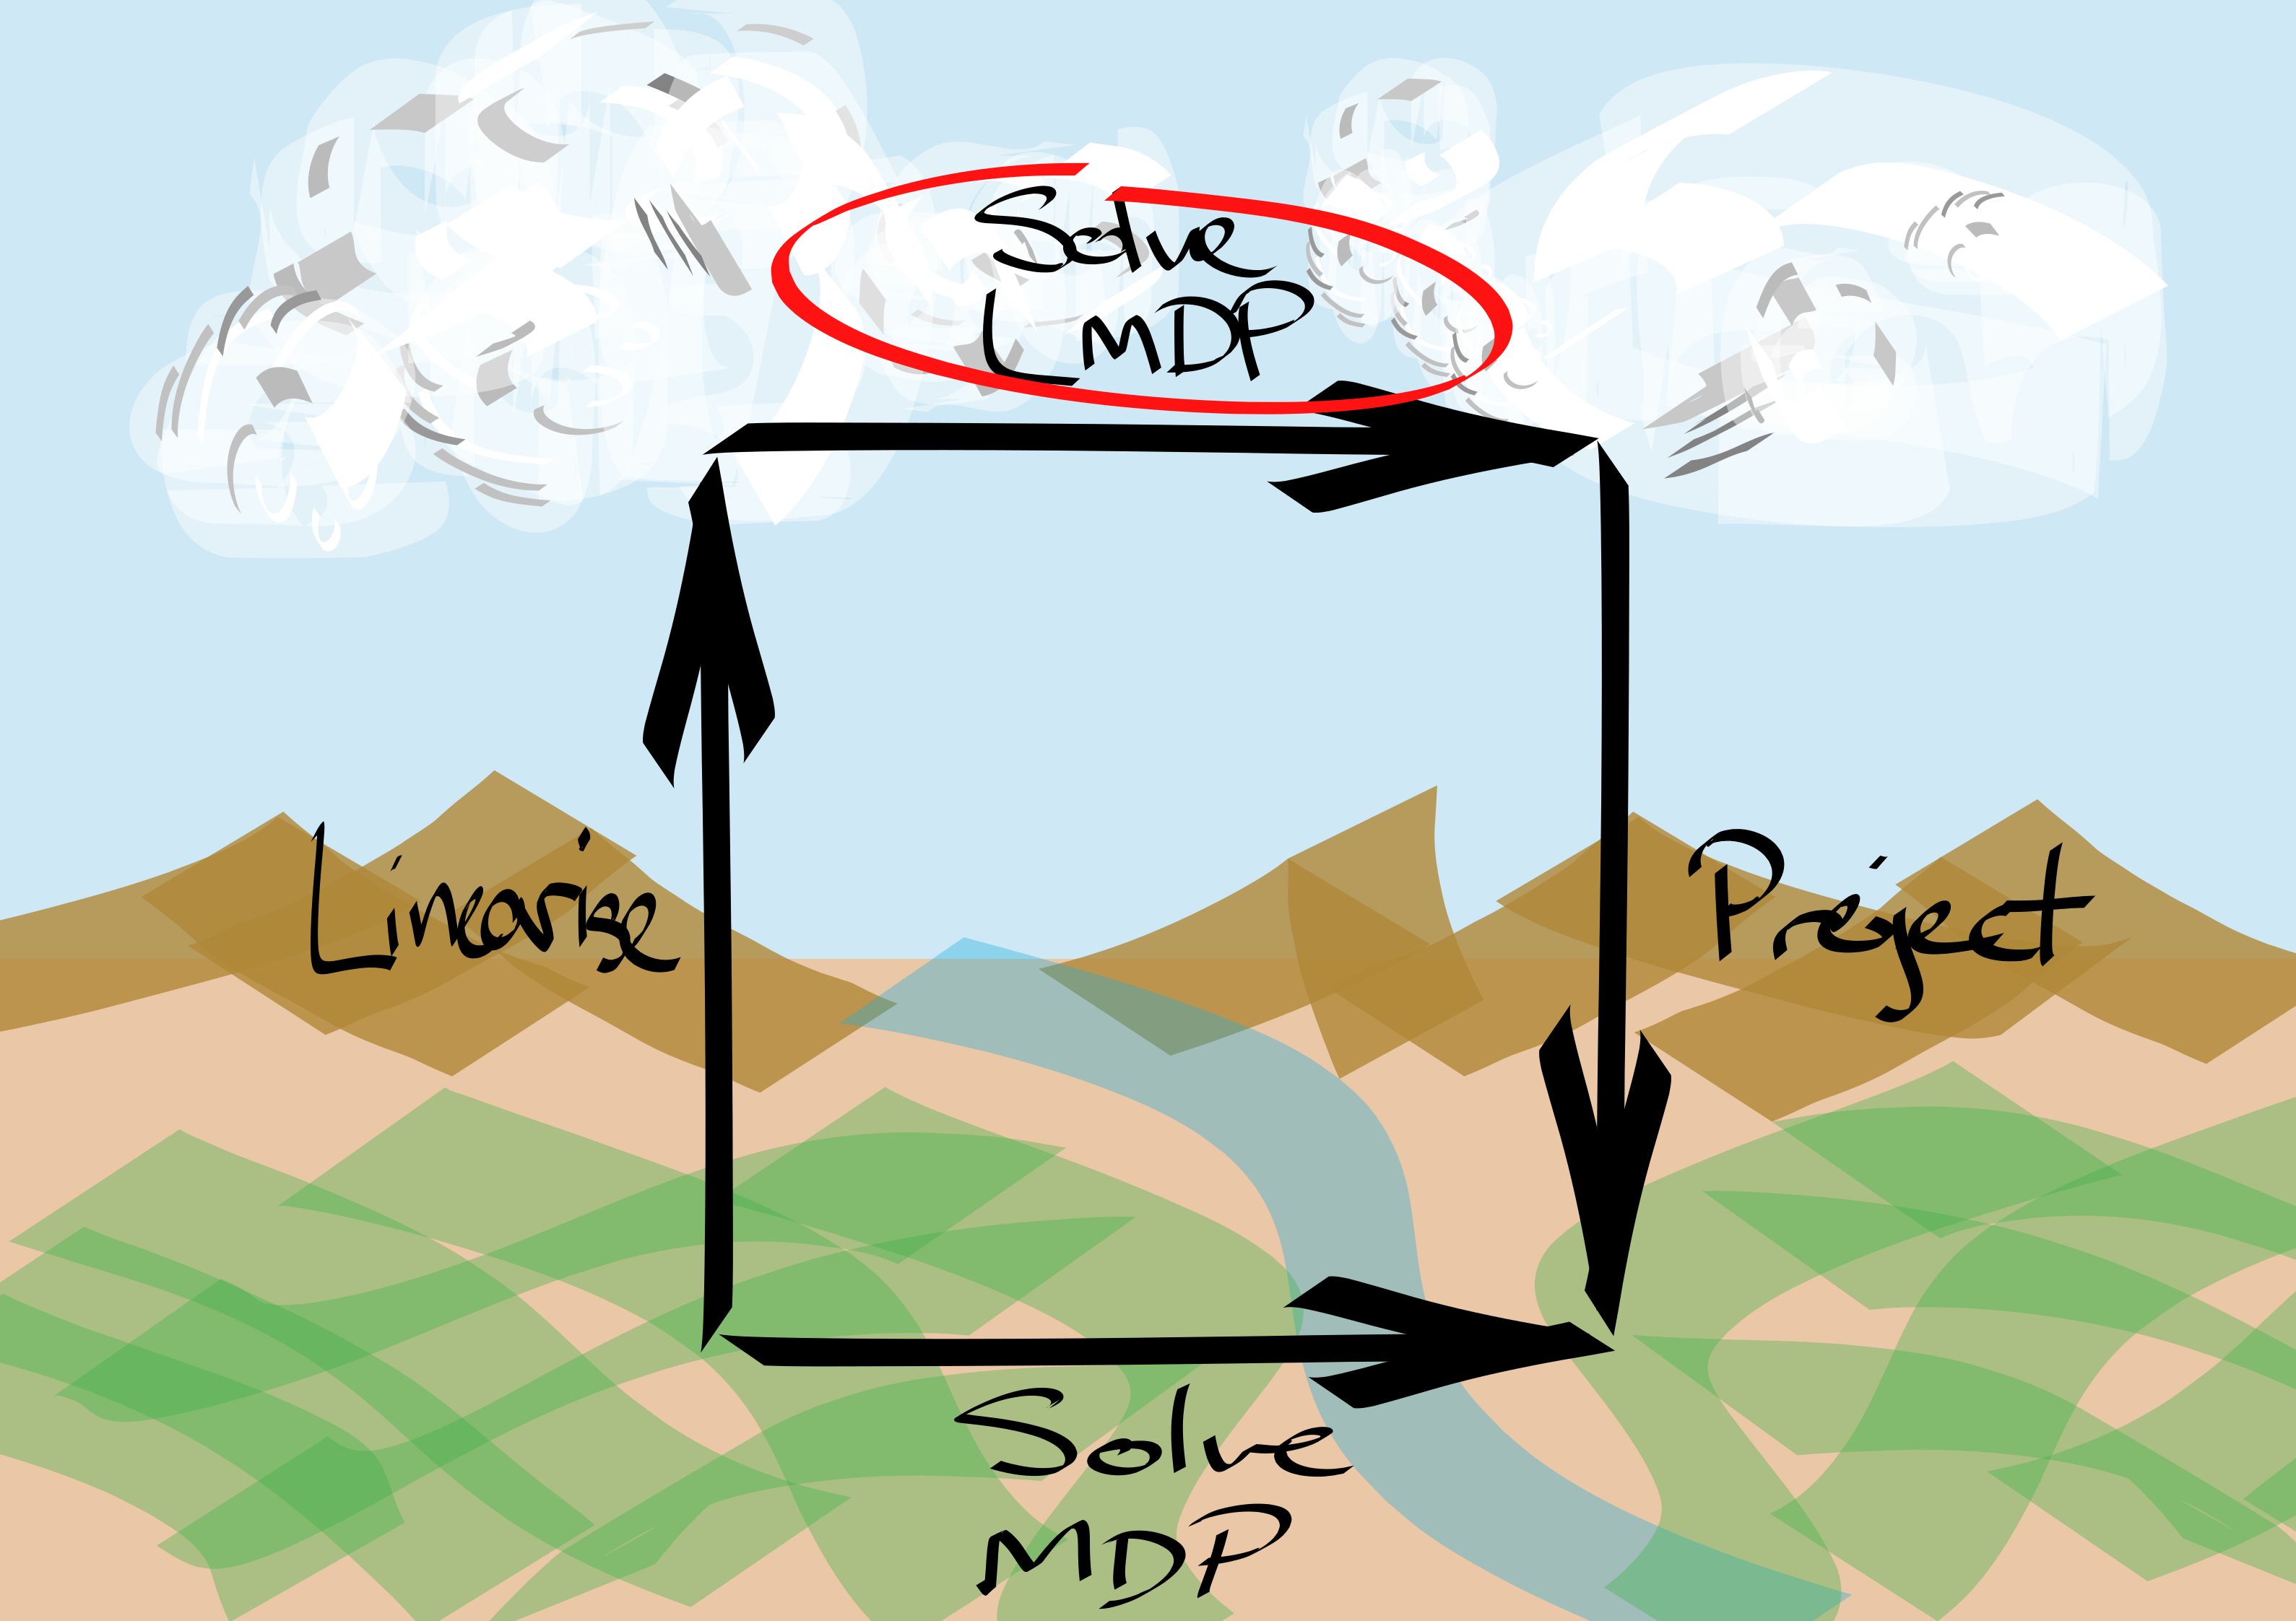
\includegraphics[width=1\textwidth,height=0.5\textheight]{../../pictures/drawings/abstract-representations-solve.png}
  \caption{'Solving the LMDP'}
\end{figure}

% intuition
To build a LMDP that acts similarly to a MDP, Todorov \cite{Todorov2006} uses a few main tricks;

\begin{itemize}
\tightlist
  \item
  they allow the agent to pick actions in the space of possible transitions, which they name controls, $u: S \to S$, rather than the action space.
  \item
  to ensure that chosen controls are possible under the given transition function, a new reward is added.
  Controls are rewarded if they are close to the 'unconstrained dynamics', $p(s' | s)$.
  \item
  rather than maximizing the cumulative reward, we maximise the exponentiated cumulative rewards.
  $\mathop{\text{max}}_{\pi} \mathop{\mathbb E}_{\zeta \sim D(\pi)} e^{R(\zeta)}$ \cite{EricWarrenFox2016}
\end{itemize}

In esscence, they are turning ...? intuition!!

Why did they need these tricks? Which ones were necessary / sufficient?

% formal definition
Putting these together, a linear markov decision process can be formulated as;
LMDP = $\{S, U, p, q, \gamma\}$. Where $p: S \to S$ is the unconditioned dynamics, and $q \in \mathbb R^{|S|}$ are state rewards.
Our goal is to find the control, $u: S \to S$, that gvies the highest exponentiated cumlative reward $z \in \mathbb R_+^{|S|}$.

\begin{align}
V(s) &= \mathop{\text{max}}_{u} q(s) - \text{KL}(u(\cdot| s) \parallel p(\cdot | s)) + \gamma \mathop{\mathbb E}_{s' \sim u(\cdot | s)} V(s') \tag{1}\\
u^{* }(\cdot | s) &= \frac{p(\cdot | s)\cdot z_{u^{* }}(\cdot)^{\gamma}}{\sum_{s'} p(s' | s) z_{u^{* }}(s')^{\gamma}} \tag{2}\\
z_{u^{* }} &= e^{q(s)}\cdot P z_{u^{* }}^{\gamma} \tag{3}
\end{align}

By definition, an LMDP is the optimisation problem in (1). After some algebra,
it can be shown (see appendix [] for a derivation) that the optimal policy has the form in (2).
And! We can solve for the value of this policy (aka we can find the optimal policy)
by solving the linear equation in (3).

\begin{displayquote}
\textit{Let's try and understand this thing we have contructed.}
\end{displayquote}

\subsubsection{Unconstrained dynamics and state rewards}

The state rewards are not capable of giving rewards for actions taken.
Rather, the differences in reward, by taking another action, is captured
by the KL divergence between the control and the unconstrained dynamics.

\begin{itemize}
\tightlist
\item
  What is their function?
\item
  What do they look like?
\end{itemize}

Does it make sense to treat the q(s) like rewards?! They reward for being
in state $s$. But cant capture action specific rewards!?

We will revisit to these questions in section [].

\subsubsection{The optimal policy}

The form of this optimal policy ...

\subsubsection{Solving for the optimal value}

Why is it we can just solve this equenction? Relation to eigen analysis?
Has nice convergence properties because it is contractive.
???

\subsection{Solving a MDP}

\begin{figure}
\centering
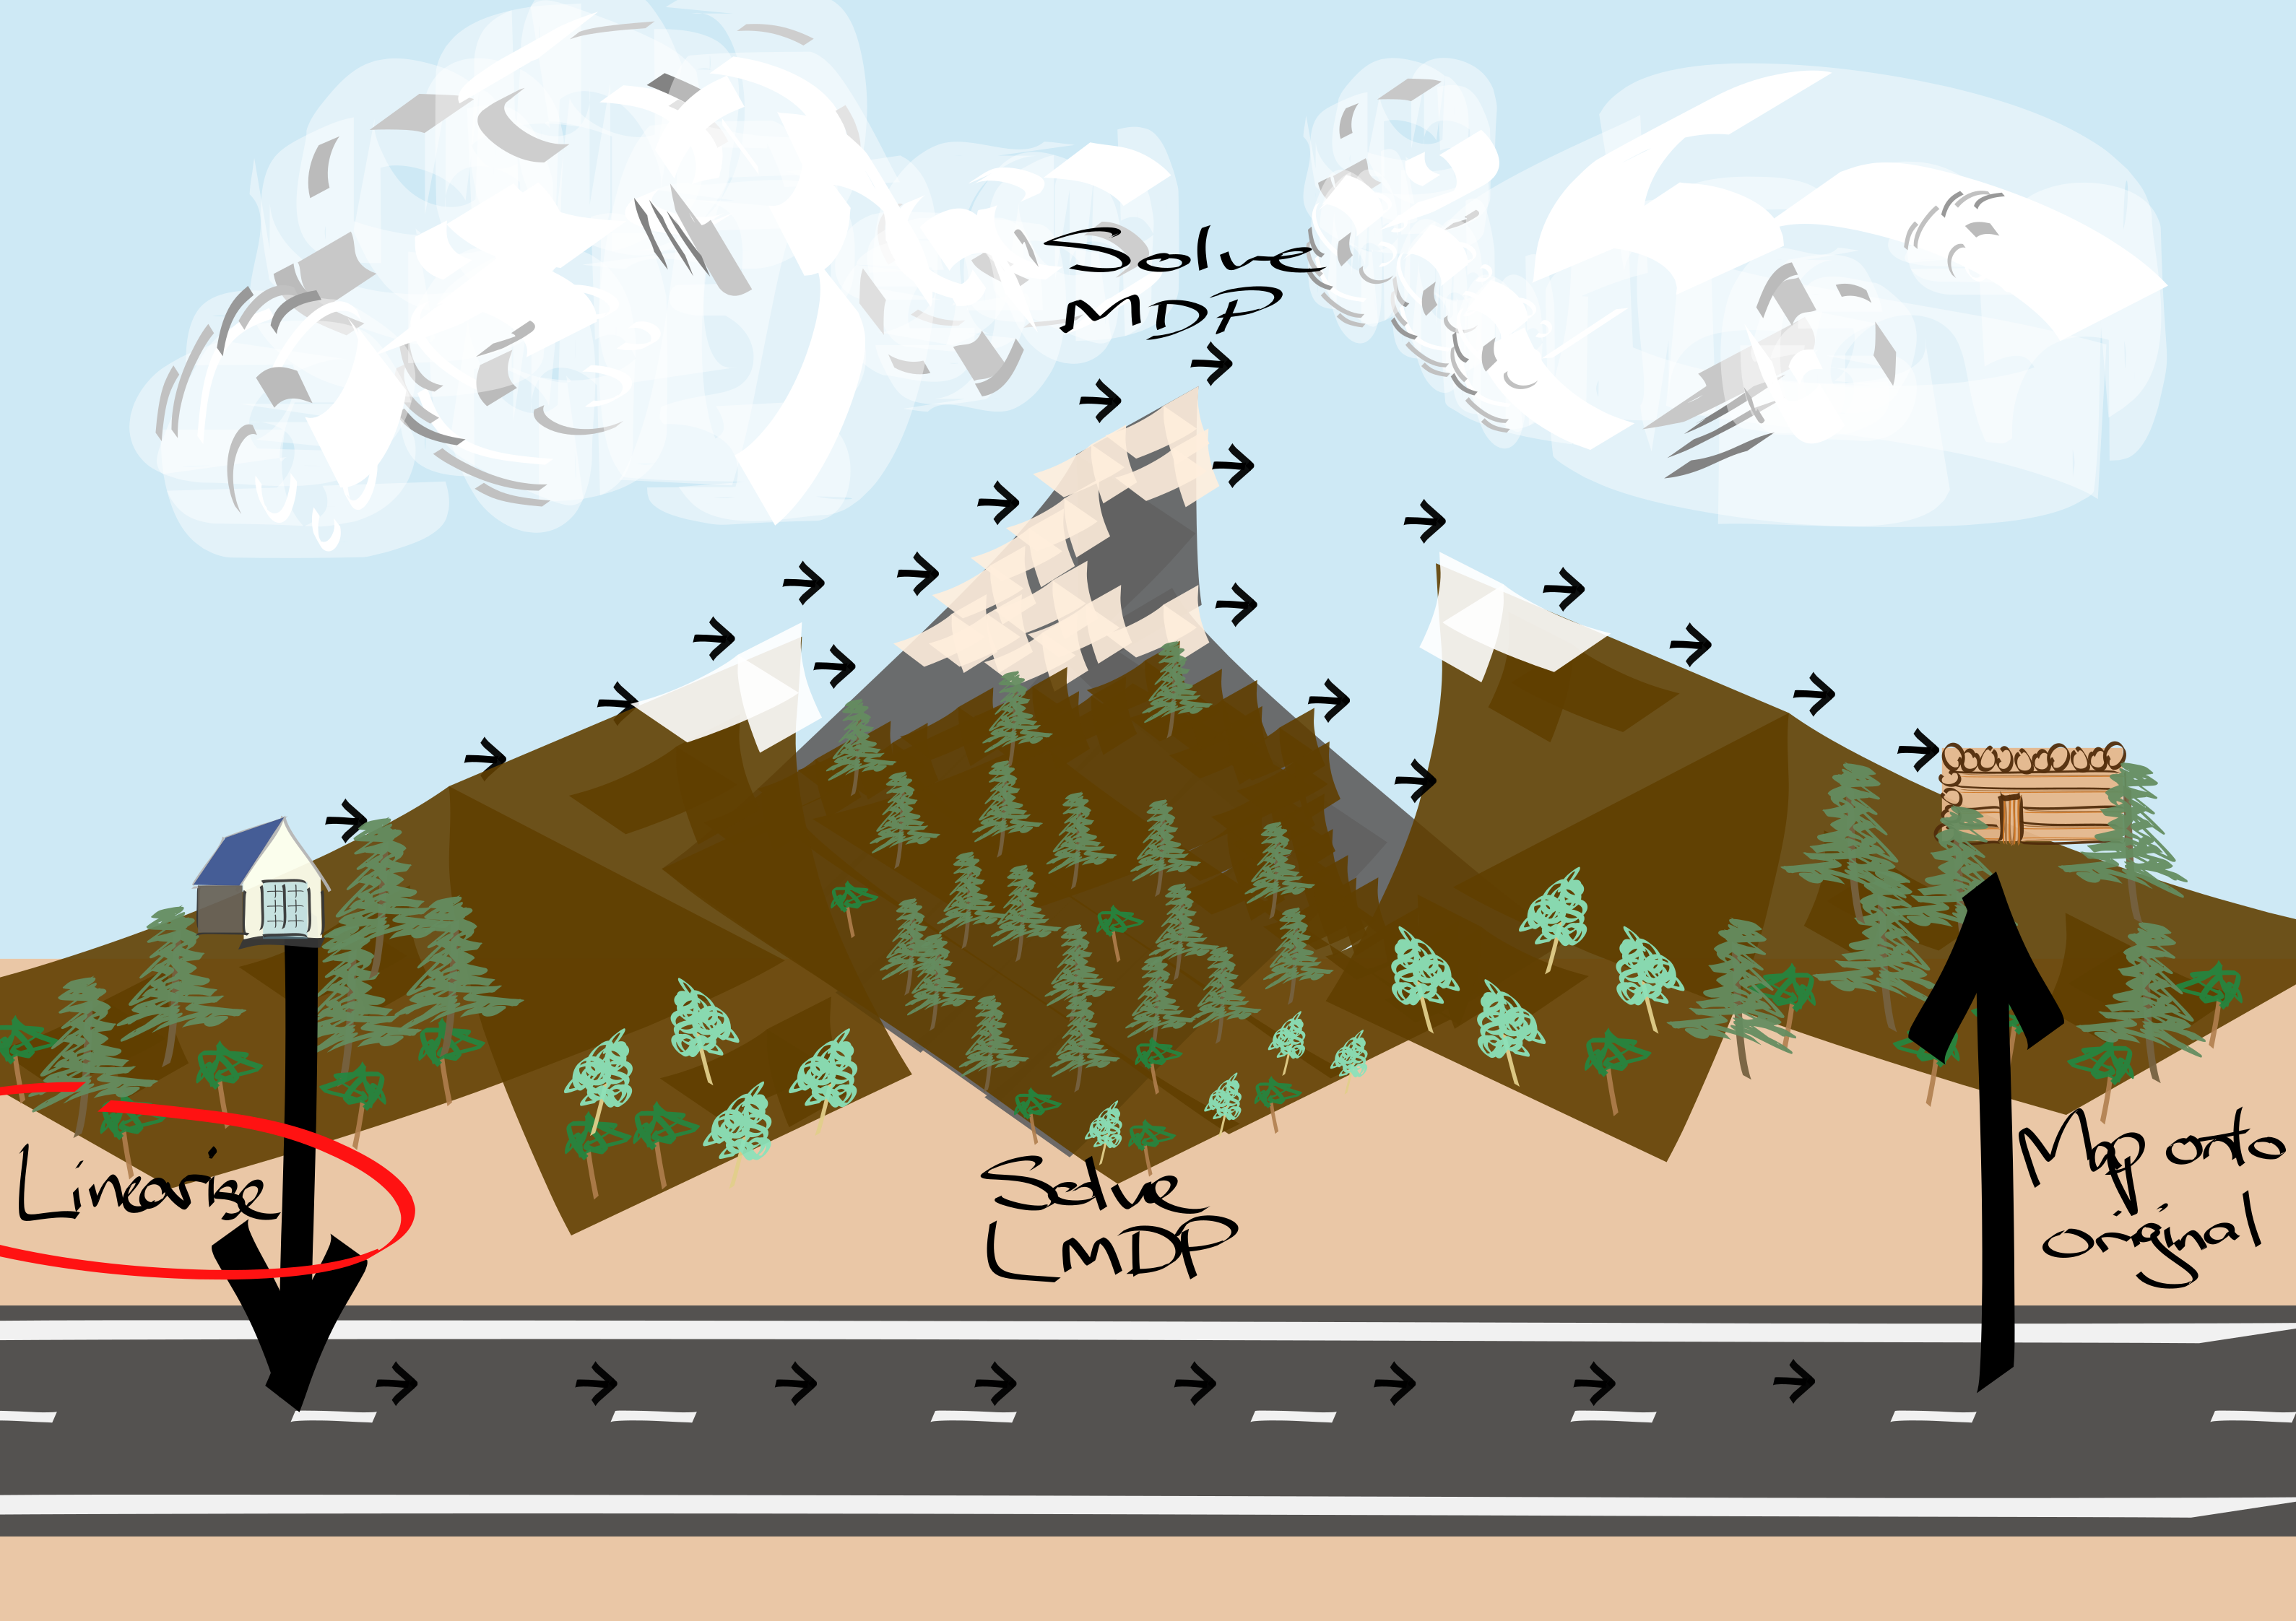
\includegraphics[width=1\textwidth,height=0.5\textheight]{../../pictures/drawings/abstract-representations-linear.png}
\caption{''}
\end{figure}

\begin{displayquote}
\textit{So, LMDPs can be easily solved. But how does solving LMDPs help us solve MDPs?}
\end{displayquote}

We want a way to transform a MDP into a LMDP, while preserving the
`structure' of the original MDP. But what do we mean by a MDP's structure?
The LMDP should; be able to represent the same transition dynamics as the original MDP (1),
and give the the same rewards was the original MDP (2). \cite{Todorov} (why? / intuition?!)

\begin{align*}
\forall s, s' \in S, \forall a \in A, \exists u_a& \;\;\text{such that;} \\
P(s' | s, a) &= u_a(s'|s)p(s'|s) \tag{1} \\
r(s, a) &= q(s) - \text{KL}(P(\cdot | s, a) \parallel u_a(\cdot| s) ) \tag{2}
\end{align*}

So, given a reward function, $r$, and a transition function, $P$,
from an MDP, we can use (1), (2) to solve for the unconditioned dynamics $p$ and a state reward $q$.
This transformation, from $P, r \to p, q$ requires $|S| \times |A|$ computations, as for each state in the
MDP \(|A|\) linear equations to solve. For more details see appendix [].

However, there are some conditions that are missing?
It might make sense to preserve the value of state-actions (3)?
And it would definitely make sense to preserve the optimal policy (4)?

\begin{align*}
\forall s, s' \in S, \forall a \in A, \forall \pi \in \Pi \\
z_{u_{\pi}}(s) = e^{v_{\pi}(s)} \tag{3} \\
P(s'|s, a) \cdot \pi^{* }(a|s) = u^{* }(s'|s) \tag{4}
\end{align*}

Where $z_{u_{\pi}}$ is the value (as evaluted by the LMDP) of the control $u_{\pi}(s'|s) = P(s'|s, a) \cdot \pi(a|s)$.

If the optimal policy is not preserved then ...

Todorov hopes that (1), (2), will be sufficient to give (4). But he does not prove it.
{\color{red}(find a quote from the paper?!?)} A potential problem that we will return to.

\begin{center}\rule{0.5\linewidth}{\linethickness}\end{center}

Initially, I thought of the unconstrained dynamics as the expected result of using random policy
$p(s' | s) = \int_a P(s' | s, a)U(a|s)$, a random walk using the transition function.
However, while this make sense intuitively, it turns out to be wrong. (more details here...)

\subsection{Decoding the optimal LMDP policy}

\begin{figure}
\centering
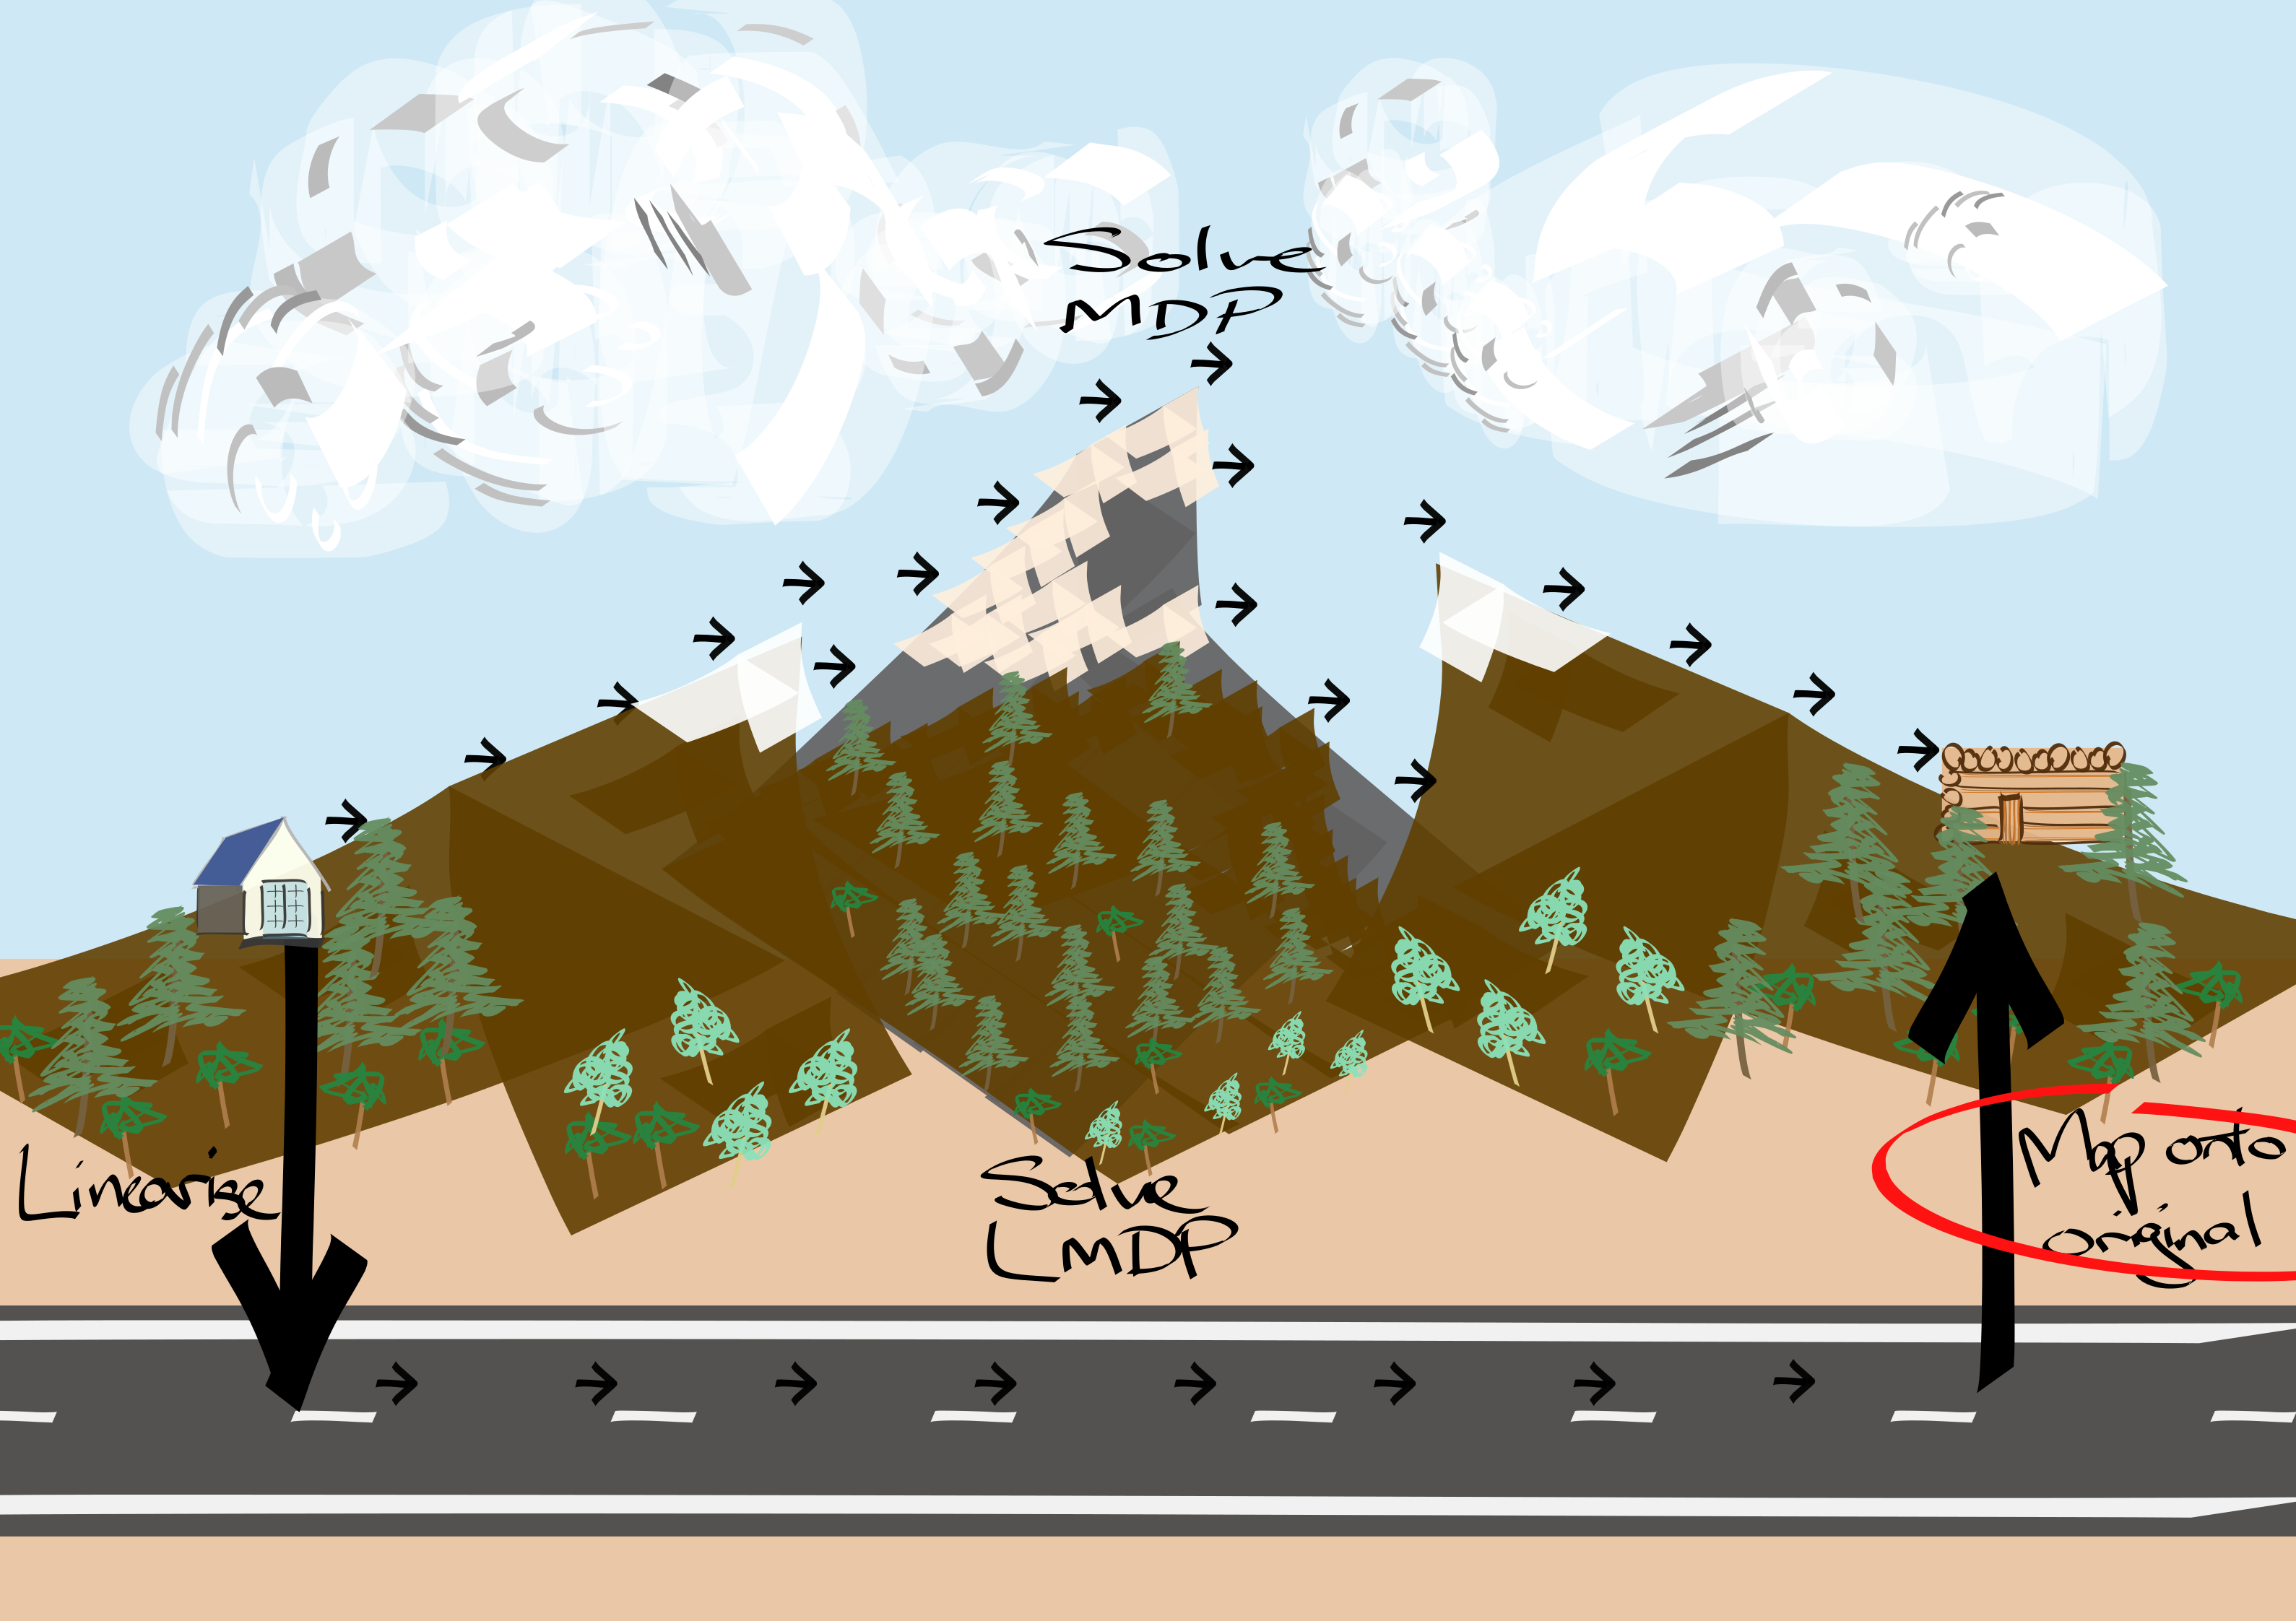
\includegraphics[width=1\textwidth,height=0.5\textheight]{../../pictures/drawings/abstract-representations-project.png}
\caption{''}
\end{figure}

We transformed our MDP into a LMDP, we can solve it. Now, how can we use $u^{* }$
to construct a policy that is optimal in the original MDP, $\pi_{u^* }$?

Here we get a glimpse at a potentially interesting abstraction.
The LMDP has disentangled the search for the optimal controls (solve the LMDP) (go to this or
that state) and the search for the optimal policy (how to actually
realise that control). This can be seen the decoding step (currently being considered). We know which
states we want to be in, the $z^{* }, u^{* }$, from solving the LMDP, but,
we do not know how to implement those controls in the original MDP.
We can formulate this decoding problem as trying to match the optimal controls (aka dynamics)
using the actions we have available.

\begin{align}
P_{\pi}(\cdot | s) = \sum_a P(\cdot | s, a) \pi(a | s) \\
\pi = \mathop{\text{argmin}}_{\pi} \text{KL}\Big(u(\cdot | s))\parallel P_{\pi}(\cdot | s)\Big)
\end{align}

This optimisation problem has very little structure.
Maybe a way to add more structure?
But it's just a special type of matrix factorisation?!? Does it have a unique minima?

Maybe this isnt enough? Do we need to add a reward sensitive part as
well?!? (but what if the actual path we take to get there has a neg
rewards?!?)

It turns out that solving \textbf{P2} is asymptotically as hard as solving a MDP.
So nothing has been gained... (proof?!?)

\subsubsection{Optimality of solutions via LMDPs}

\begin{quote}
\textit{Do these two paths lead to the same place?}
\end{quote}

One of the main questions we have not addressed yet is; if we solve the
MDP directly, or linearise, solve and project, do we end up in the same
place? This is a question about the completeness of our abstraction. Can
our abstraction represent (and find) the same solutions that the
original can?

$\epsilon_{\pi}$ will tell us if the solutions are different. But What we really care about
is whether the value is different. We might not care if the optimal control yields a policy that is different from the optimal policy, as long as the
 policy via optimal control achieves high performance. We can measure this with $\epsilon_{V}$.

\begin{align*}
\epsilon_{\pi} &= \text{KL}\Big(u(\cdot | s))\parallel P_{\pi}(\cdot | s)\Big) \\
\epsilon_{V} &= \parallel V_{\pi^{* }} - V_{\pi_{u^{* }}} \parallel_{\infty}
\end{align*}

To evaluate $V_{\pi_{u^{* }}}$, the value of the decoded optimal control, we can
set $P_{\pi} = u^{* }$. And solve $V = (I - \gamma P_{\pi})^{-1} \cdot r_{\pi}$.
However, $r_{u^{* }}$ doesnt really make sense as the reward is action
dependent. We would like to be able to calculate $r_{\pi_{u^{* } }}$, but we dont
explicity know \(\pi_{u^{* }}\). By solving $(I - \gamma P_{\pi^{* }})^{-1} \dot r$
we get the state-action values, or $Q$ values of the optimal control.

Results...

\begin{figure}
\centering
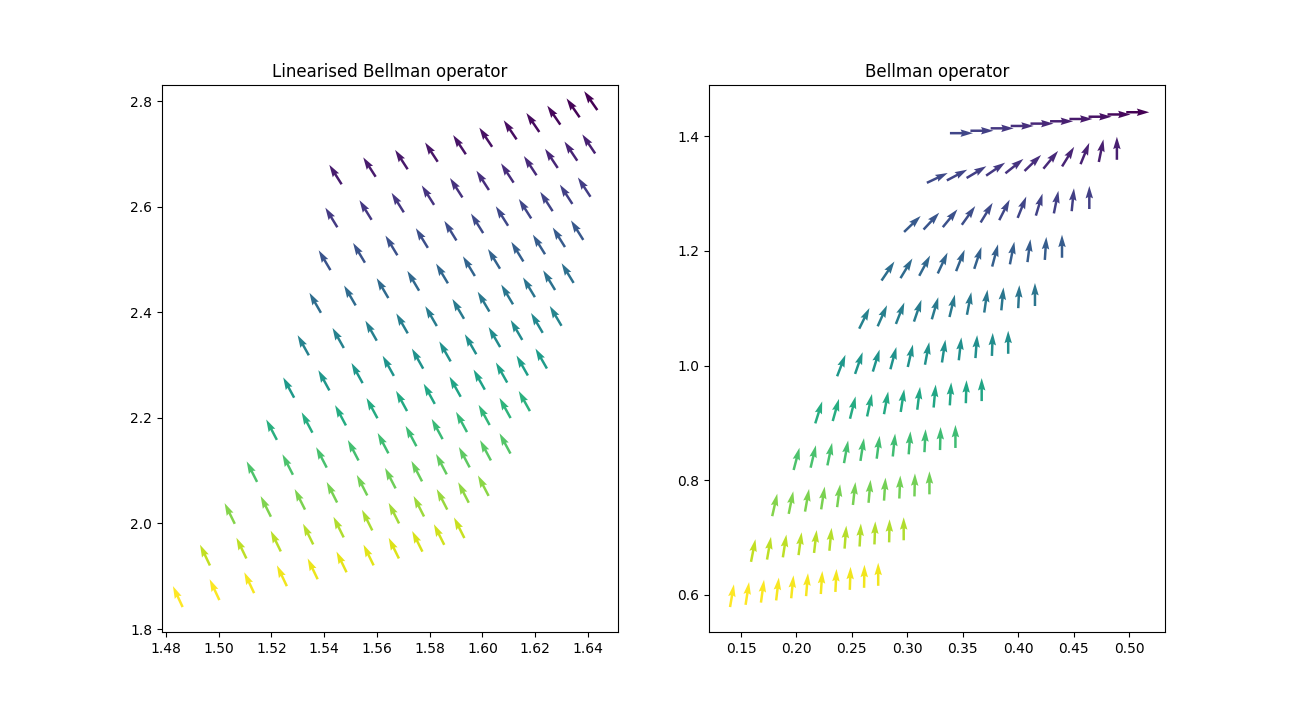
\includegraphics[width=0.75\textwidth,height=0.5\textheight]{../../pictures/figures/LBO_BO.png}
\caption{For the same MDP, shown is a comparison of the linear temporal difference operator (left), versus the true, Bellman, temporal difference operator (right). As expected, the Bellman temporal difference operator points towards the optimal value. But, ther linear temporal difference operator points elsewhere...}
\end{figure}

\begin{figure}
\centering
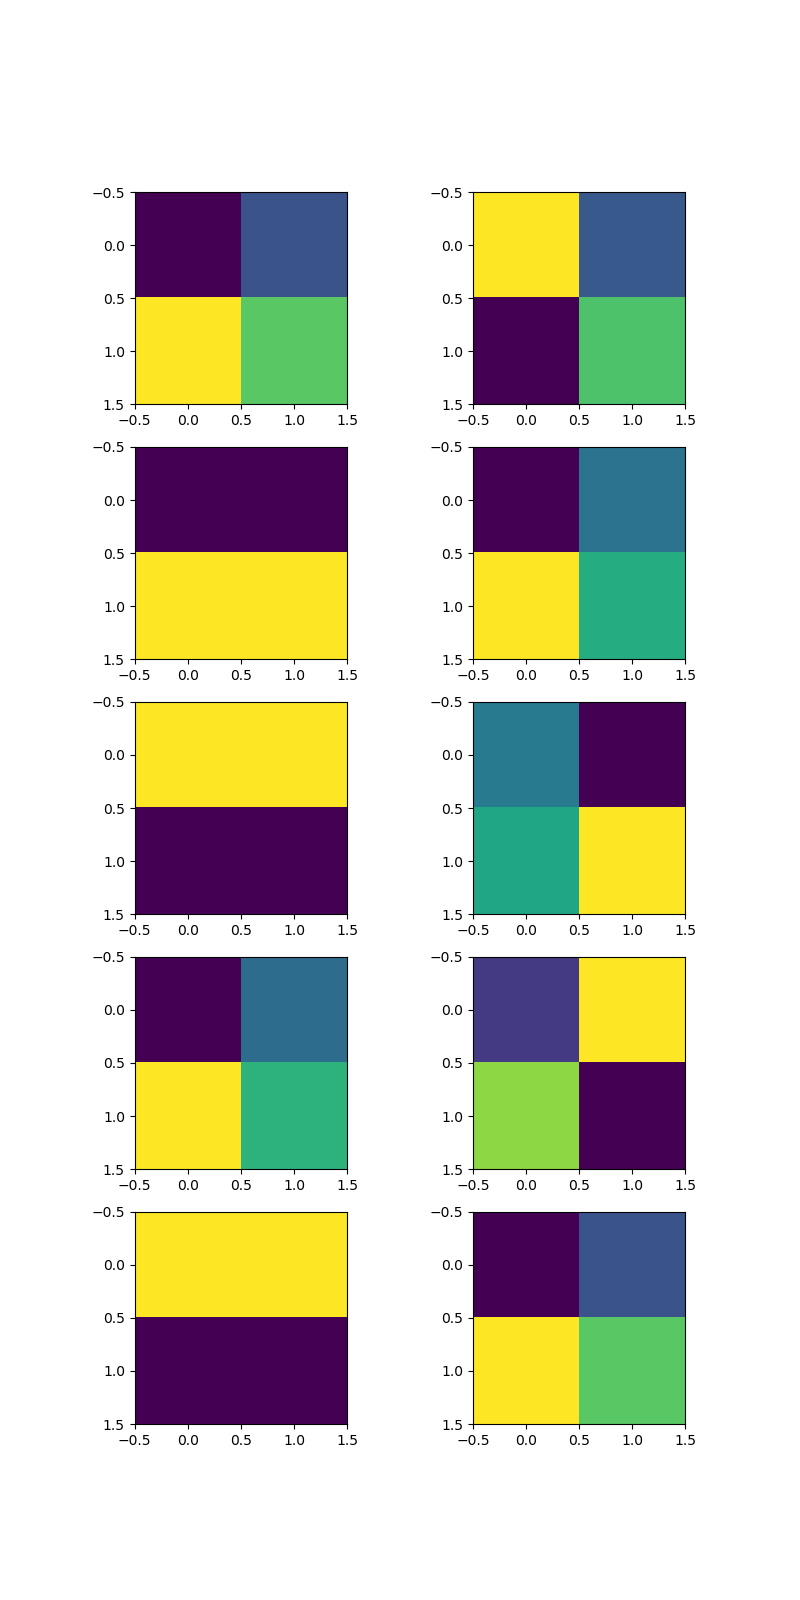
\includegraphics[width=0.5\textwidth,height=0.75\textheight]{../../pictures/figures/lmdp_mdp_optimal_dynamics.png}
\caption{A comparison between the optimal control (LMDP) and the optimal policy (MDP).}
\end{figure}

\subsubsection{The complexity of solutions via LMDPs}

\begin{quote}
Is my path actually shorter?
\end{quote}

The whole point of this abstraction was to make the problem easier to
solve. So has it actually made it any easier?

The complexity of solving our abstraction can be broken down into the
three steps;

\begin{itemize}
\tightlist
\item
  linearisation: \(|S| \times \text{min}(|S|,|A|)^{2.3}\)
\item
  solve the LMDP: \(\text{min}(|S|,|A|)^{2.3}\)
\item
  project back: \(???\)
\end{itemize}

Given that the first step was not passed, optimality. We did not continue this characterisation.

\subsection{Scaling to more complex problems}

Now that we have some evidence that this LMDP solution strategy makes
sense, it efficiently (see \href{}{complexity}) yields high value (see
\href{}{optimality}) policies. We want to test it out on some real world
problems. But the real world isn't as nice as the setting we have been
working in. There are a few added complexities;

\begin{itemize}
\tightlist
\item
  sample based / incremental
\item
  large / cts state spaces
\item
  sparse rewards
\end{itemize}

So now that we have explored LMDPs, how can we extract their nice
properties into an architecture that might scale to more complex
problems: larger state spaces and action spaces, sparse rewards,
\ldots{}?

\subsubsection{Incremental implementation}

Generalise to a more complex problem. We are only given samples. A first
step to tackling more complex problems.


\subsubsection{Model based}

Learn \(p, q\) based on samples.

\begin{align}
\mathcal L(\theta, \phi) = \mathop{\mathbb E}_{s, a,} \bigg[ r(s, a) - q_\theta(s) + \text{KL}(p_\phi(\cdot | s) \parallel P(\cdot | s, a)) \bigg]\\
\mathcal L(\theta, \phi) = \mathop{\mathbb E}_{s, r, s'} \bigg[r - q_\theta(s) - p_\phi(s' | s) \log \frac{1}{ p_\phi(s' | s)} \bigg] \\
\end{align}

\begin{center}\rule{0.5\linewidth}{\linethickness}\end{center}

Ok. Lets take a different approach. \textbf{Q:} Why is it a bad idea to
try to do incremental RL with this linearisation trick? Not sure.

\begin{center}\rule{0.5\linewidth}{\linethickness}\end{center}

Alternative perspective. The high value trajectories are the most likely
ones.

\subsubsection{Distributions over states}

What if we wanted to approximate these distributions? Generalise subgoal
methods to work with distributions? The distribution could be
constructed via; parzen window / GMM, neural flow, ?!.

Connections to distributional RL?

Questions

\begin{itemize}
\tightlist
\item
  What is p(s'\textbar{}s)!?!?
\item
  Want some examples of MDPs they cannot solve.
\item
  What is the relationship to other action embedding strategies?
\item
  How does p(s'\textbar{}s) bias the controls found??? I can imagine the
  unconstrained dynamics acting as a prior and prefering some controls
  over others.
\item
  If we have m states and n actions. Where m
  \textgreater{}\textgreater{} n. Then \(u(s'|s)\) is much larger than
  \(\pi(a|s)\). Also, \(u(s'|s)\) should be low rank?!
  \(u_{s's} = \sum_a u_a \alpha_a u_a^T\)
\end{itemize}



Refs \cite{Todorov2006,Todorov2009,Zhong,Zhonga,Dvijotham,Wozabal}



\begin{figure}
\centering
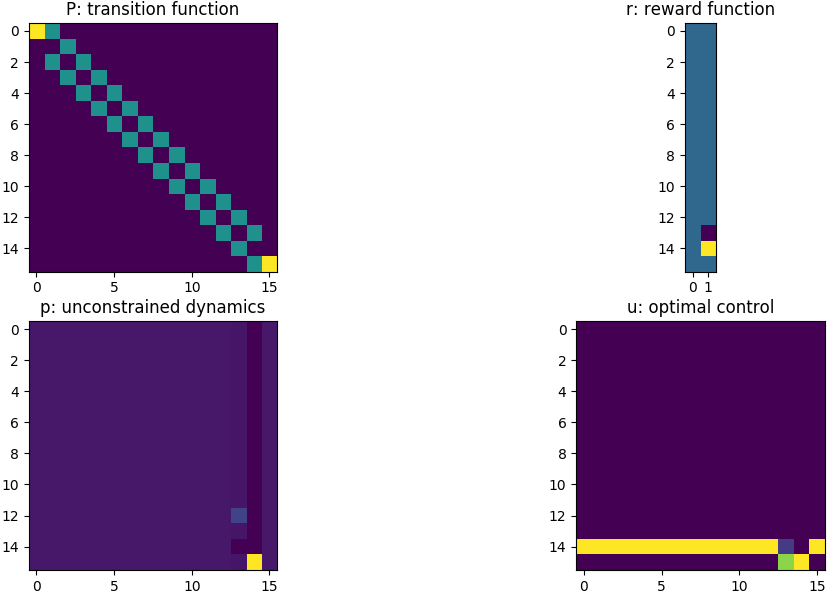
\includegraphics[width=1\textwidth,height=0.35\textheight]{../../pictures/figures/chain-test-zero-rewards.png}
\caption{A chain problem with zero reward on all states except the last two.
The optimal control to this problem is not sensible: in every state, jump to the state with positive reward.
However, it is not possible to make those transitions as }
\end{figure}

\begin{figure}
\centering
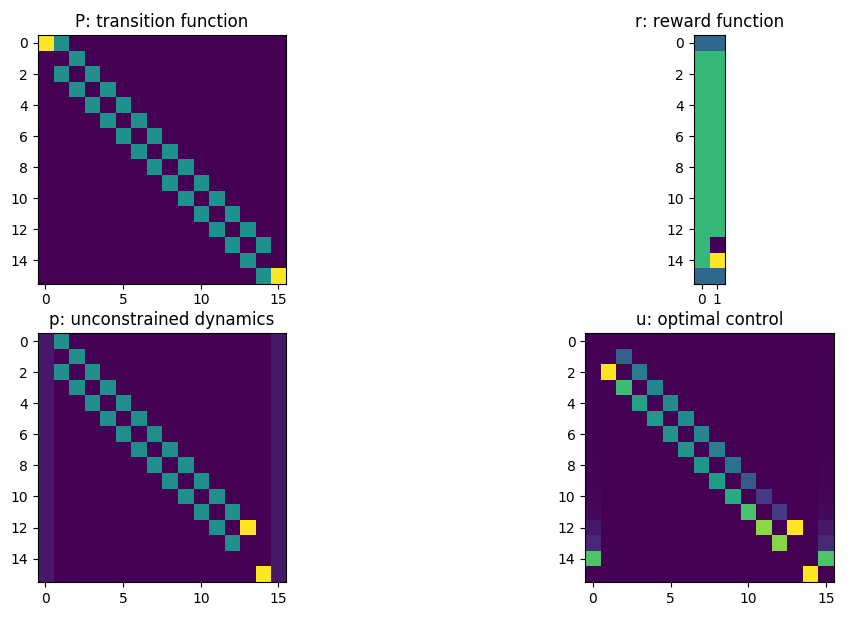
\includegraphics[width=1\textwidth,height=0.35\textheight]{../../pictures/figures/chain-test-pos-rewards.png}
\caption{A chain problem with positive rewards applied to all states.}
\end{figure}

\begin{figure}
\centering
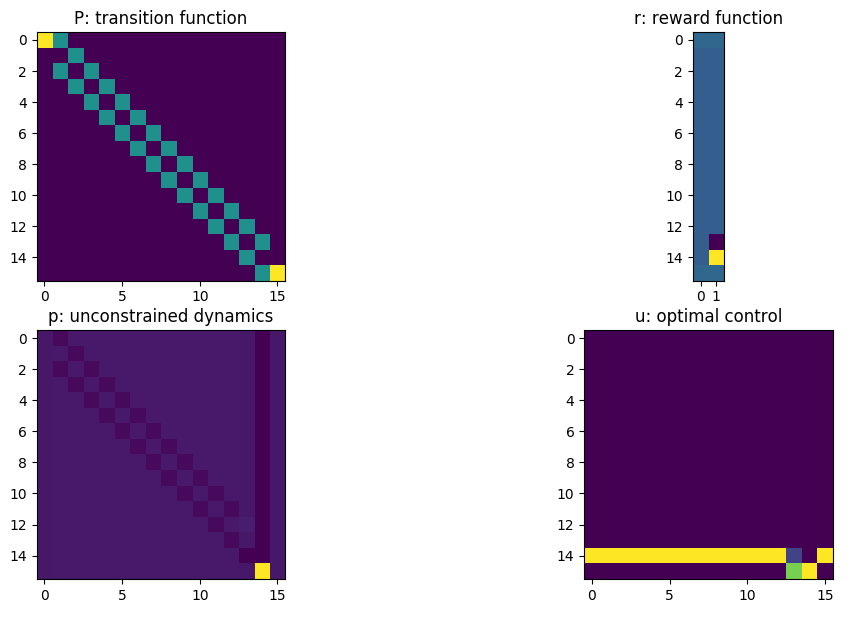
\includegraphics[width=1\textwidth,height=0.35\textheight]{../../pictures/figures/chain-test-neg-rewards.png}
\caption{A chain problem with negative rewards applied to all states}
\end{figure}

The point is, it is not entierly clear how to embed an MDP into a LMDP.
